% Options for packages loaded elsewhere
\PassOptionsToPackage{unicode}{hyperref}
\PassOptionsToPackage{hyphens}{url}
%
\documentclass[
  man]{apa6}
\usepackage{amsmath,amssymb}
\usepackage{lmodern}
\usepackage{iftex}
\ifPDFTeX
  \usepackage[T1]{fontenc}
  \usepackage[utf8]{inputenc}
  \usepackage{textcomp} % provide euro and other symbols
\else % if luatex or xetex
  \usepackage{unicode-math}
  \defaultfontfeatures{Scale=MatchLowercase}
  \defaultfontfeatures[\rmfamily]{Ligatures=TeX,Scale=1}
\fi
% Use upquote if available, for straight quotes in verbatim environments
\IfFileExists{upquote.sty}{\usepackage{upquote}}{}
\IfFileExists{microtype.sty}{% use microtype if available
  \usepackage[]{microtype}
  \UseMicrotypeSet[protrusion]{basicmath} % disable protrusion for tt fonts
}{}
\makeatletter
\@ifundefined{KOMAClassName}{% if non-KOMA class
  \IfFileExists{parskip.sty}{%
    \usepackage{parskip}
  }{% else
    \setlength{\parindent}{0pt}
    \setlength{\parskip}{6pt plus 2pt minus 1pt}}
}{% if KOMA class
  \KOMAoptions{parskip=half}}
\makeatother
\usepackage{xcolor}
\usepackage{graphicx}
\makeatletter
\def\maxwidth{\ifdim\Gin@nat@width>\linewidth\linewidth\else\Gin@nat@width\fi}
\def\maxheight{\ifdim\Gin@nat@height>\textheight\textheight\else\Gin@nat@height\fi}
\makeatother
% Scale images if necessary, so that they will not overflow the page
% margins by default, and it is still possible to overwrite the defaults
% using explicit options in \includegraphics[width, height, ...]{}
\setkeys{Gin}{width=\maxwidth,height=\maxheight,keepaspectratio}
% Set default figure placement to htbp
\makeatletter
\def\fps@figure{htbp}
\makeatother
\setlength{\emergencystretch}{3em} % prevent overfull lines
\providecommand{\tightlist}{%
  \setlength{\itemsep}{0pt}\setlength{\parskip}{0pt}}
\setcounter{secnumdepth}{-\maxdimen} % remove section numbering
% Make \paragraph and \subparagraph free-standing
\ifx\paragraph\undefined\else
  \let\oldparagraph\paragraph
  \renewcommand{\paragraph}[1]{\oldparagraph{#1}\mbox{}}
\fi
\ifx\subparagraph\undefined\else
  \let\oldsubparagraph\subparagraph
  \renewcommand{\subparagraph}[1]{\oldsubparagraph{#1}\mbox{}}
\fi
\newlength{\cslhangindent}
\setlength{\cslhangindent}{1.5em}
\newlength{\csllabelwidth}
\setlength{\csllabelwidth}{3em}
\newlength{\cslentryspacingunit} % times entry-spacing
\setlength{\cslentryspacingunit}{\parskip}
\newenvironment{CSLReferences}[2] % #1 hanging-ident, #2 entry spacing
 {% don't indent paragraphs
  \setlength{\parindent}{0pt}
  % turn on hanging indent if param 1 is 1
  \ifodd #1
  \let\oldpar\par
  \def\par{\hangindent=\cslhangindent\oldpar}
  \fi
  % set entry spacing
  \setlength{\parskip}{#2\cslentryspacingunit}
 }%
 {}
\usepackage{calc}
\newcommand{\CSLBlock}[1]{#1\hfill\break}
\newcommand{\CSLLeftMargin}[1]{\parbox[t]{\csllabelwidth}{#1}}
\newcommand{\CSLRightInline}[1]{\parbox[t]{\linewidth - \csllabelwidth}{#1}\break}
\newcommand{\CSLIndent}[1]{\hspace{\cslhangindent}#1}
\ifLuaTeX
\usepackage[bidi=basic]{babel}
\else
\usepackage[bidi=default]{babel}
\fi
\babelprovide[main,import]{english}
% get rid of language-specific shorthands (see #6817):
\let\LanguageShortHands\languageshorthands
\def\languageshorthands#1{}
% Manuscript styling
\usepackage{upgreek}
\captionsetup{font=singlespacing,justification=justified}

% Table formatting
\usepackage{longtable}
\usepackage{lscape}
% \usepackage[counterclockwise]{rotating}   % Landscape page setup for large tables
\usepackage{multirow}		% Table styling
\usepackage{tabularx}		% Control Column width
\usepackage[flushleft]{threeparttable}	% Allows for three part tables with a specified notes section
\usepackage{threeparttablex}            % Lets threeparttable work with longtable

% Create new environments so endfloat can handle them
% \newenvironment{ltable}
%   {\begin{landscape}\centering\begin{threeparttable}}
%   {\end{threeparttable}\end{landscape}}
\newenvironment{lltable}{\begin{landscape}\centering\begin{ThreePartTable}}{\end{ThreePartTable}\end{landscape}}

% Enables adjusting longtable caption width to table width
% Solution found at http://golatex.de/longtable-mit-caption-so-breit-wie-die-tabelle-t15767.html
\makeatletter
\newcommand\LastLTentrywidth{1em}
\newlength\longtablewidth
\setlength{\longtablewidth}{1in}
\newcommand{\getlongtablewidth}{\begingroup \ifcsname LT@\roman{LT@tables}\endcsname \global\longtablewidth=0pt \renewcommand{\LT@entry}[2]{\global\advance\longtablewidth by ##2\relax\gdef\LastLTentrywidth{##2}}\@nameuse{LT@\roman{LT@tables}} \fi \endgroup}

% \setlength{\parindent}{0.5in}
% \setlength{\parskip}{0pt plus 0pt minus 0pt}

% Overwrite redefinition of paragraph and subparagraph by the default LaTeX template
% See https://github.com/crsh/papaja/issues/292
\makeatletter
\renewcommand{\paragraph}{\@startsection{paragraph}{4}{\parindent}%
  {0\baselineskip \@plus 0.2ex \@minus 0.2ex}%
  {-1em}%
  {\normalfont\normalsize\bfseries\itshape\typesectitle}}

\renewcommand{\subparagraph}[1]{\@startsection{subparagraph}{5}{1em}%
  {0\baselineskip \@plus 0.2ex \@minus 0.2ex}%
  {-\z@\relax}%
  {\normalfont\normalsize\itshape\hspace{\parindent}{#1}\textit{\addperi}}{\relax}}
\makeatother

% \usepackage{etoolbox}
\makeatletter
\patchcmd{\HyOrg@maketitle}
  {\section{\normalfont\normalsize\abstractname}}
  {\section*{\normalfont\normalsize\abstractname}}
  {}{\typeout{Failed to patch abstract.}}
\patchcmd{\HyOrg@maketitle}
  {\section{\protect\normalfont{\@title}}}
  {\section*{\protect\normalfont{\@title}}}
  {}{\typeout{Failed to patch title.}}
\makeatother

\usepackage{xpatch}
\makeatletter
\xapptocmd\appendix
  {\xapptocmd\section
    {\addcontentsline{toc}{section}{\appendixname\ifoneappendix\else~\theappendix\fi\\: #1}}
    {}{\InnerPatchFailed}%
  }
{}{\PatchFailed}
\keywords{keywords\newline\indent Word count: X}
\DeclareDelayedFloatFlavor{ThreePartTable}{table}
\DeclareDelayedFloatFlavor{lltable}{table}
\DeclareDelayedFloatFlavor*{longtable}{table}
\makeatletter
\renewcommand{\efloat@iwrite}[1]{\immediate\expandafter\protected@write\csname efloat@post#1\endcsname{}}
\makeatother
\usepackage{csquotes}
\ifLuaTeX
  \usepackage{selnolig}  % disable illegal ligatures
\fi
\IfFileExists{bookmark.sty}{\usepackage{bookmark}}{\usepackage{hyperref}}
\IfFileExists{xurl.sty}{\usepackage{xurl}}{} % add URL line breaks if available
\urlstyle{same} % disable monospaced font for URLs
\hypersetup{
  pdftitle={Testing the JD-R theory via O*Net definitional specification},
  pdfauthor={Alicia A. Stachowski1 \& John T. Kulas2},
  pdflang={en-EN},
  pdfkeywords={keywords},
  hidelinks,
  pdfcreator={LaTeX via pandoc}}

\title{Testing the JD-R theory via O*Net definitional specification}
\author{Alicia A. Stachowski\textsuperscript{1} \& John T. Kulas\textsuperscript{2}}
\date{}


\shorttitle{Hindrances-Resources Interaction}

\authornote{

Add complete departmental affiliations for each author here. Each new line herein must be indented, like this line.

Enter author note here.

The authors made the following contributions. Alicia A. Stachowski: Conceptualization, Writing - Original Draft Preparation, Writing - Review \& Editing; John T. Kulas: Writing - Review \& Editing.

Correspondence concerning this article should be addressed to Alicia A. Stachowski, Postal address. E-mail: \href{mailto:stachowskia@uwstout.edu}{\nolinkurl{stachowskia@uwstout.edu}}

}

\affiliation{\vspace{0.5cm}\textsuperscript{1} University of Wisconsin - Stout\\\textsuperscript{2} eRg}

\abstract{%
This project explored the role of resources on the demand-strain relationship through the lens of O*Net derived job characteristics. When dissociating demands into challenges and hindrances, we did find tentative support for resources moderating the hindrance-strain relationship.
}



\begin{document}
\maketitle

The Job Demands-Resources Theory (JD-R, Demerouti et al., 2001) has received wide support across contexts and varied research questions. We extend the literature by 1) exploring the interaction between job demands and resources on the experience of strain using O*Net job characteristics and 2) considering also the appraisal of demands as challenge or hindrance stressors. Here, respondents made a series of evaluations that used: direct O*Net terminology (both descriptor and response option), and JD-R influenced ratings of challenge and hindrance stressors. Prior to a description of results, a brief overview of both the JD-R theory, the stress appraisal process, and O*Net, is provided.

\hypertarget{the-job-demands-resources-theory}{%
\subsection{The Job Demands-Resources Theory}\label{the-job-demands-resources-theory}}

The job demands-resources theory is an expansion of the well-studied job demands-resources model (Demerouti et al., 2001). One of the major advantages of the job demands-resources theory is that it allows us to model both work environment and job characteristics (which are thoroughly documented across many jobs within O*Net) via \emph{resources} and \emph{demands}. Resources are defined as physical, psychological, social, or organizational aspects of the job that may help an employee achieve work goals, reduce job demands, or promote personal growth and development (Demerouti et al., 2001). Demands, on the other hand, include components of a job that require sustained effort, and as such, produce psychological or physiological strain (e.g., high work pressure; Demerouti et al. (2001)).

Cognitively, the perception of an element of one's job as a resource or demand activates one of two unique processes: health impairment (resulting from demands) or motivation (resulting from resources, Bakker \& Demerouti, 2014). Demanding job characteristics are frequently associated with negative outcomes (e.g., Bakker et al., 2003), whereas job characteristics deemed resources have been associated with positive organizational outcomes like engagement and motivation (Bakker et al., 2007). However, a related line of research emphasizes a further distinction between two types of demands - that of \emph{challenge} and \emph{hindrance} demands, suggesting that employees may evaluate stressors in different ways.

\hypertarget{the-subjective-nature-of-demands-and-resources-the-role-of-appraisal}{%
\subsection{The Subjective Nature of Demands and Resources: The Role of Appraisal}\label{the-subjective-nature-of-demands-and-resources-the-role-of-appraisal}}

The stress/strain literature speaks to the key consideration of the way employees appraise situations or circumstances - in this case, our focus will be on work characteristics. The transactional theory of stress and coping suggests that people cognitively appraise stimuli in their environments on a continuous basis (Lazarus \& Folkman, 1984). For example, two employees both informed that they need to step in and assume the responsibilities of a coworker in their absence may react differently to this job demand. One may feel quite paralyzed by the added or novel tasks, while the other may embrace it as an exciting new challenge. The terms associated with the two different appraisals of the same stressor are ``challenge'' and ``hindrance'' demands (Cavanaugh et al., 2000) Challenge demands promote mastery, personal growth, and future gains. Hindrance demands, by definition, inhibit growth, learning and goal achievement. Perhaps not surprisingly, challenge stressors are typically associated with positive outcomes, whereas hindrance stressors are associated with more negative outcomes (e.g., Cavanaugh et al., 2000). Our focus here will be on the connection between hindrance demands specifically, and their association with reported strain. More specifically, our interest here is whether or not the negative hindrance association we typically observe between demands and strain can be buffered by perceived resources.

Searle and Auton (2015) note that much of our research on workplace demands is based on \emph{a priori} classifications of demands. For instance, we assume that generally, time pressure is a negative demand on an employee. However, the stress/strain experience, or process, described early on by Lazarus and Folkman (1984) is grounded in the assumption that individual appraisals of stressors/demands vary. Their transactional theory of stress and coping states that people continuously appraise stimuli in their environments. An appraisal is the cognitive process whereby meaning is assigned to a stimulus. If a stimulus is appraised as a stressor (threat, challenge, potentially harmful), emotional distress leads to coping of some kind. This action to cope is also associated with another appraisal about the outcome itself and the process continues if the outcomes are not appraised as favorable (Lazarus \& Folkman, 1984). As such, the stress appraisal process suggests that classifying a job characteristic or environmental condition as an objective demand or resource might be in error.

We next consider the empirical evidence on the subjective nature of demands and resources. First, as hinted at above, some research suggests that job demands and resources may not be universally appraised or assigned as such. Starting with job demands, Webster et al. (2011) studied workload, role ambiguity, and role conflict, and found that while each could be appraised primarily as a challenge or hindrance demand, they could also simultaneously be perceived as being \emph{both} a challenge and hindrance to different degrees. While their study did not include resources, it does document individual differences in how people may perceive stressors at work. Additionally, although not the primary focus of their paper, Sonnega et al. (2018) compared self-reported (subjective) ratings of job demands with more objective ratings of the same characteristics, finding that perceptions of characteristics may be subject to a greater level of individual difference than we tend to think.

While the above two studies provide evidence for variability in how workers view \emph{demands}, Schmitz et al. (2019) went on to further capture subjective and objective \emph{resources} in their study of retirement. They found only very small associations between subjective and objective measures for the ``typically implicated'' as resources variables of: 1) autonomy, 2) recognition of work, and 3) decision making freedom, again suggesting universal classification may not be appropriate. Downes et al. (2021) meta-analysis addresses this reality in depth, although a broader current elaboration is beyond the scope of this SIOP presentation.

Thus, while it is cleaner to be able to categorize job characteristics as \emph{either} a demand or a resource, the above research suggests that an individual's (perhaps unique) appraisal is at least occasionally an important consideration. It is quite possible that one person experiences high work pressure (commonly cited as a demand in the literature) as a hindrance stressor and thus experiences strain, and another thrives in a fast-paced pressured role and would thus find the environment motivating. In order to account for this possibility of ``non-exclusivity'', we asked our respondents to rate all relevant job characteristics in terms of their status as hindrances, challenges, and resources.

\hypertarget{value-of-consulting-onet}{%
\subsection{Value of consulting O*Net}\label{value-of-consulting-onet}}

The Occupational Information Network (O*NET; onetonline.org) contains a fairly comprehensive description of occupations (Peterson et al., 2001). This widely accessed database houses hundreds of standardized and occupation-specific descriptors for the majority of occupations within the United States, and these descriptions are frequently updated. These data, and the tools provided for public consumption on the website (e.g., Career Exploration Tools, ``My Next Move'', Toolkit for Business) are frequently used by counselors, students, human resources departments, and researchers to assist interested or curious job-seekers discover the nature of work as well as skills and training typically required for different occupations. It is also often useful to employers by providing them with information that may be helpful in a job analysis context. For the current study, we focused on statements taken from O*NET's \href{https://www.O*NETonline.org/find/descriptor/result/4.A.1.b.3}{``activity'' and ``context'' classifications} (e.g., items related to characteristics of work such as how often a worker interacts with others or engages in physical labor). From a job analytic lens, these descriptors are written more broadly than a task statement, and would most likely be classified by most job analysts as ``responsibilities''.

\hypertarget{current-study-and-hypotheses}{%
\section{Current Study and Hypotheses}\label{current-study-and-hypotheses}}

The data we describe here represents a subset taken from a larger study on JD-R theory and its integration within the O*NET framework. For SIOP, we specifically investigate Proposition 3 of the JD-R model - that job resources can buffer the impact of job demands on strain. The interaction between job resources and demands has been heavily studied with regard to a range of outcomes. For example Bakker et al. (2010) found that resources (e.g., learning opportunities, autonomy, leader support) predicted both task enjoyment and organizational commitment even under conditions of high demands. In fact, a rather large body of empirical evidence supports this assertion (e.g., see Bakker \& Demerouti, 2017 for a historical review). Much of the research, however, has focused on stress/strain and burnout outcomes. For example, Bakker et al. (2005) found that job resources lessen the impact of demands on burnout in a large sample of employees working in higher education, and Xanthopoulou et al. (2007) found similar patterns in a sample of home care organization employees.

Our unique contribution in the current study is in whether or not \emph{perceptions} of demands as hindrances or challenges are related to experienced strain, and whether or not this relationship is moderated by the presence of resources. We do have some existing evidence that this occurs with other outcomes beyond strain. For example, Tadić et al. (2015) found that daily hindrance job demands were negatively related to both positive affect and engagement in a sample of primary school teachers. Daily job resources, in this sample, buffered the relationships between hindrances and affect and engagement. With the current investigation, we propose that greater perceived resources generally, as opposed to daily, would also buffer the relationship between perceived hindrance stressors and, in this, case, experienced strain. The following two predictions are made:

\begin{quote}
\emph{H1}. There is a positive relationship between perceived hindrance stressors and strain.
\end{quote}

\begin{quote}
\emph{H2}. The relationship between mean perceived hindrances and strain will be moderated by resources such that this relationship is diminished as perceived resources increase.
\end{quote}

\hypertarget{methods}{%
\section{Methods}\label{methods}}

Data were collected through Prolific, a data collection platform. An email was sent to a random subset of all eligible participants in the Prolific respondent pool, notifying them about their eligibility for the study based on demographic information. Eligibility requirements included being 18+ and holding either a full-time or part-time job. Participants then voluntarily chose to respond to the survey. The survey was conducted online via Qualtrics with an estimated completion time of 40-45 minutes. Participants were asked to think about their primary job while answering the survey, and the items they were presented with depended on the specific job characteristics they initially specified. Thus, if a respondent indicated that a characteristic was not part of their job, they were not subsequently asked to rate the level of resource, challenge, or hindrance for that characteristic. For characteristics that \emph{were} implicated as being relevent for their job, they were then asked to report how much a characteristic was a resource, and then how much each characteristic was a hindrance, and finally, how much each item was a challenge. Participants were compensated for their participation in this study in the amount of six dollars through Prolific.

\hypertarget{participants}{%
\subsection{Participants}\label{participants}}

785 individuals initially accessed the survey link. Of those 785, several indicated that they were not interested after learning more about the project, had more than 200 missing responses, or had 20 or more identical consecutive sequential responses. Any individual respondent who fell into any of these three areas of concern was removed from the initial data frame, resulting in a final realized sample of 568. 13.57\% of these individuals had been in their referent job less than 6 months, 19.20\% between 6 months and a year, 49.12\% between one and five years, 13.27\% between 5 and 10 years, and 4.87\% more than 10 years. Their ages ranged from 18 to 65 with an average of 28.18 years old (\emph{SD} = 7.53). Over half (52.58\%) identified as female, and 46.83\% identified as male.

\hypertarget{materials}{%
\section{Materials}\label{materials}}

\hypertarget{resources-and-hindrances.}{%
\subsubsection{Resources and Hindrances.}\label{resources-and-hindrances.}}

To guage resources and hindrances, we used 98 statements taken directly from O*Net's ``activity'' and ``context'' classifications. Each of the 98 descriptors has potentially unique response categories, but scaling was consistently 1 (low) to 5 (high). Subsequent to self-evaluations regarding whether or not the characteristic was applicable to one's job, the respondents were asked to rate germane elements in terms of it's experience as a resource (``\ldots this aspect of your job is a resource that can be functional in achieving work goals, reduce job demands, or stimulate personal growth/development''), challenge, (\ldots this aspect of your job is a challenge that can promote mastery, personal growth, or future gains'') as well as hindrance (``\ldots this aspect of your job is a hindrance that can inhibit personal growth, learning, and work goal attainment''). For each category (e.g., resources), a mean score was computed that indicated the across items that applied to one's role, and thus, mean scores could range from 1 to 5.

\hypertarget{strain.}{%
\subsubsection{Strain.}\label{strain.}}

Three items taken from the Copenhagen Psychosocial Questionnaire (Burr et al., 2019) captured strain (an example item is: ``How often have you had problems relaxing because of your job?''). Responses were made on a 5-point scale ranging from ``not at all'' to ``all the time''. Alpha was .85 in this sample.

\hypertarget{results}{%
\section{Results}\label{results}}

\begin{figure}
\centering
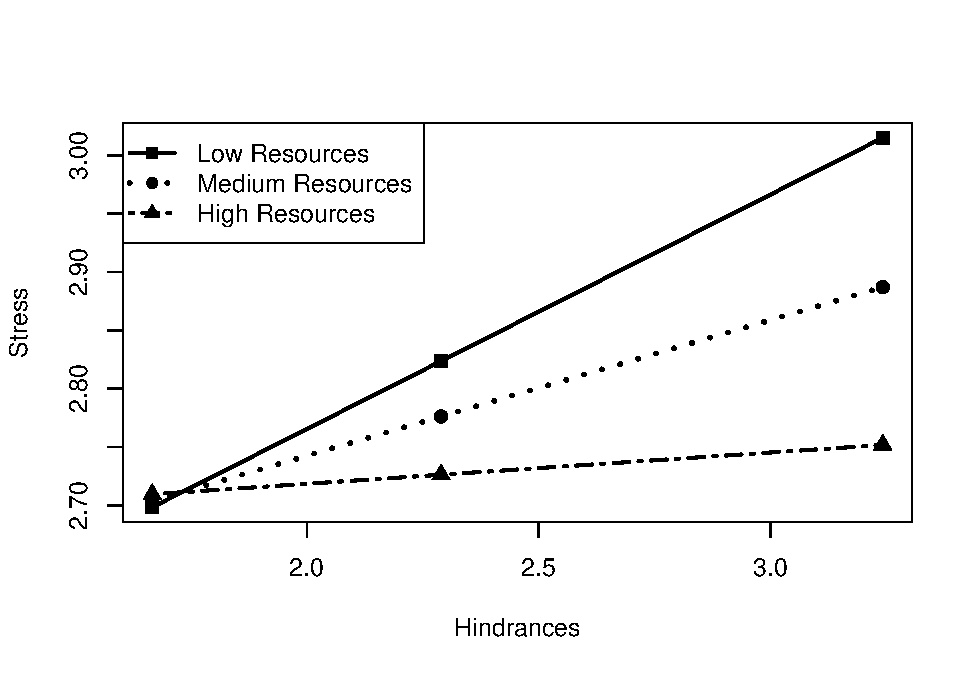
\includegraphics{SIOP_PROCESS_files/figure-latex/analyses-1.pdf}
\caption{\label{fig:analyses}Interaction between hindrances and resources as predictors of stress}
\end{figure}

\begin{table}[tbp]

\begin{center}
\begin{threeparttable}

\caption{\label{tab:cortab}Challenge, hindrance, and resource bivariate correlations with stress.}

\begin{tabular}{llllll}
\toprule
 & \multicolumn{1}{c}{1} & \multicolumn{1}{c}{2} & \multicolumn{1}{c}{3} & \multicolumn{1}{c}{$M$} & \multicolumn{1}{c}{$SD$}\\
\midrule
1. Stress & - &  &  & 2.81 & 0.89\\
2. Challenge & -.05 & - &  & 3.73 & 0.48\\
3. Hindrance & .09* & -.19*** & - & 2.40 & 0.75\\
4. Resource & -.08 & .75*** & -.24*** & 3.73 & 0.47\\
\bottomrule
\end{tabular}

\end{threeparttable}
\end{center}

\end{table}

Following data cleaning and preparation, we computed correlations among the study variables. See Table \ref{tab:cortab}. With regard to H1, which predicted a positive association between perceived hindrance stressors and strain, a small positive relationship was observed, \emph{r} = .09, \emph{p} \textless{} .05. Thus, ``weak'' support was found for H1.

\begin{table}[tbp]

\begin{center}
\begin{threeparttable}

\caption{\label{tab:table}Results from a regression analysis examining the moderation of resources on the relationship between hindrance demands and strain}

\begin{tabular}{lllll}
\toprule
Component & \multicolumn{1}{c}{coeff} & \multicolumn{1}{c}{SE} & \multicolumn{1}{c}{t} & \multicolumn{1}{c}{p}\\
\midrule
Constant & 1.27 & 1.01 & 1.26 & 0.21\\
Hindrance (X) & 0.83 & 0.40 & 2.07 & 0.04\\
Resource (W) & 0.33 & 0.25 & 1.32 & 0.19\\
Hindrance x Resource & -0.19 & 0.10 & -1.87 & 0.06\\
\bottomrule
\end{tabular}

\end{threeparttable}
\end{center}

\end{table}

Next, to explore H2, a moderated regression including hindrances, resources, and the interaction between them was done using PROCESS, version 4.1.1 (Hayes, 2022, see Table \ref{tab:table}). First, the overall regression model including mean hindrances, mean resources, and the interaction between the two variables was significant, \(F_{(3, 564)}\) = 3.29, \emph{p} = .020. The interaction between hindrance and resources (uncentered) revealed that the relationship between hindrances and strain was conditional on resources, \(F_{(3, 564)}\) = 3.51, \emph{p} = .061, providing marginal support for H2. As can be seen in Figure \ref{fig:analyses}, those with fewer resources show a much stronger positive relationship between hindrances and strain than those with more resources. As such, these results provide some evidence that resources may moderate the relationship between hindrance demands and subsequent levels of strain.

\hypertarget{discussion}{%
\section{Discussion}\label{discussion}}

The primary goal of this project was to further explore the role of perceived resources on the hindrance-strain relationship using O*Net characteristics. While we have plentiful evidence that resources can buffer the effects of a variety of job demands on burnout, this project focuses on subjective experiences of resources and demands, focusing on demands rated as challenges and hindrances, as well as focusing on the outcome of \emph{strain}. As expected, the results suggest a positive relationship between perceived hindrances and strain (H1). While intuitive, it is important to replicate this finding before we explore the impact of perceived resources, which arguably, is something that employers may have more leverage to control than hindrance stressors.

Second, the results serve to support the assertion that resources change the relationship between hindrances and strain such that the connection between the two is diminished as resources increase (H2). While not hypothesized or presented above, the authors did also run a regression on the \emph{challenge}-strain relationship with resources as a moderator, with the assumption that resources would not moderate the relationship. The findings, indeed, did not indicate a moderated relationship in this case. It appears that resources are of benefit particularly when hindrances are present. In particular, the Job-demands Resources Theory (Demerouti et al., 2001) suggests that resources would buffer the negative impact between demands and strain, and by extension, given the more traditional conceptualization of demands would be aligned with hindrance demands.
These findings have implications worth considering. In a practical sense within the workplace, they speak to the ever present need to ensure employees have sufficient resources. Our project focused on the characteristics of one's work specifically, and in line with the literature cited above, studied the ratings or perceptions of resources and demands to account for individual differences in the way employees appraise components of their work. From a academic research standpoint, these findings integrate three related literatures: the job-demands resources, stress appraisal, and challenge-hindrance framework to examine the experience of employees across jobs - specifically, the way that resources and hindrance demands interact on the experience of strain. Results align with what all three theories/frameworks would suggest.

\hypertarget{limitations-and-future-directions}{%
\subsection{Limitations and Future Directions}\label{limitations-and-future-directions}}

Here, we note a number of limitations, but also provide additional directions for future research on this topic. First, while the use of O*Net items is a strength of the paper, practical considerations limited the number of job characteristics we could include in our survey. Because our focus was on O*Net items and our procedure was time and effort intensive, we were unable to inquire about other forms of resources (e.g., supervisor or coworker support) or demands. Thus, future study could explore these sources of support as resources and perhaps even compare the importance of various types of resources and their role in reducing the influence of hindrance stressors using O*Net characteristics. Is it overall perceptions of having more resources that makes up for hindrances, or could it be that certain resources carry more weight? Second, our focus here was on the outcome of strain, but it may also be of value to consider what the interaction between ratings of O*Net characteristics as resources and hindrances looks like on other outcomes of interest in a work context (e.g., commitment, motivation, engagement, intent to quit).

\newpage

\hypertarget{references}{%
\section{References}\label{references}}

\begingroup
\setlength{\parindent}{-0.5in}
\setlength{\leftskip}{0.5in}

\hypertarget{refs}{}
\begin{CSLReferences}{1}{0}
\leavevmode\vadjust pre{\hypertarget{ref-bakker2014job}{}}%
Bakker, A. B., \& Demerouti, E. (2014). Job demands--resources theory. \emph{Wellbeing: A Complete Reference Guide}, 1--28.

\leavevmode\vadjust pre{\hypertarget{ref-bakker2017job}{}}%
Bakker, A. B., \& Demerouti, E. (2017). Job demands--resources theory: Taking stock and looking forward. \emph{Journal of Occupational Health Psychology}, \emph{22}(3), 273.

\leavevmode\vadjust pre{\hypertarget{ref-bakker2005job}{}}%
Bakker, A. B., Demerouti, E., \& Euwema, M. C. (2005). Job resources buffer the impact of job demands on burnout. \emph{Journal of Occupational Health Psychology}, \emph{10}(2), 170.

\leavevmode\vadjust pre{\hypertarget{ref-bakker2003dual}{}}%
Bakker, A. B., Demerouti, E., \& Schaufeli, W. (2003). Dual processes at work in a call centre: An application of the job demands--resources model. \emph{European Journal of Work and Organizational Psychology}, \emph{12}(4), 393--417.

\leavevmode\vadjust pre{\hypertarget{ref-bakker2007job}{}}%
Bakker, A. B., Hakanen, J. J., Demerouti, E., \& Xanthopoulou, D. (2007). Job resources boost work engagement, particularly when job demands are high. \emph{Journal of Educational Psychology}, \emph{99}(2), 274.

\leavevmode\vadjust pre{\hypertarget{ref-bakker2010beyond}{}}%
Bakker, A. B., Van Veldhoven, M., \& Xanthopoulou, D. (2010). Beyond the demand-control model: Thriving on high job demands and resources. \emph{Journal of Personnel Psychology}, \emph{9}(1), 3.

\leavevmode\vadjust pre{\hypertarget{ref-burr_third_2019}{}}%
Burr, H., Berthelsen, H., Moncada, S., Nübling, M., Dupret, E., Demiral, Y., Oudyk, J., Kristensen, T. S., Llorens, C., Navarro, A., Lincke, H.-J., Bocéréan, C., Sahan, C., Smith, P., \& Pohrt, A. (2019). The {Third} {Version} of the {Copenhagen} {Psychosocial} {Questionnaire}. \emph{Safety and Health at Work}, \emph{10}(4), 482--503. \url{https://doi.org/10.1016/j.shaw.2019.10.002}

\leavevmode\vadjust pre{\hypertarget{ref-cavanaugh2000empirical}{}}%
Cavanaugh, M. A., Boswell, W. R., Roehling, M. V., \& Boudreau, J. W. (2000). An empirical examination of self-reported work stress among US managers. \emph{Journal of Applied Psychology}, \emph{85}(1), 65.

\leavevmode\vadjust pre{\hypertarget{ref-demerouti2001job}{}}%
Demerouti, E., Bakker, A. B., Nachreiner, F., \& Schaufeli, W. B. (2001). The job demands-resources model of burnout. \emph{Journal of Applied Psychology}, \emph{86}(3), 499.

\leavevmode\vadjust pre{\hypertarget{ref-downes2021incorporating}{}}%
Downes, P. E., Reeves, C. J., McCormick, B. W., Boswell, W. R., \& Butts, M. M. (2021). Incorporating job demand variability into job demands theory: A meta-analysis. \emph{Journal of Management}, \emph{47}(6), 1630--1656.

\leavevmode\vadjust pre{\hypertarget{ref-hayes2022}{}}%
Hayes, A. F. (2022). \emph{Introduction to mediation, moderation, and conditional process analysis: A regression-based approach} (3rd ed.). The Guilford Press.

\leavevmode\vadjust pre{\hypertarget{ref-lazarus1984stress}{}}%
Lazarus, R. S., \& Folkman, S. (1984). \emph{Stress, appraisal, and coping}. Springer publishing company.

\leavevmode\vadjust pre{\hypertarget{ref-peterson2001understanding}{}}%
Peterson, N. G., Mumford, M. D., Borman, W. C., Jeanneret, P. R., Fleishman, E. A., Levin, K. Y., Campion, M. A., Mayfield, M. S., Morgeson, F. P., Pearlman, K., et al. (2001). Understanding work using the occupational information network (o* NET): Implications for practice and research. \emph{Personnel Psychology}, \emph{54}(2), 451--492.

\leavevmode\vadjust pre{\hypertarget{ref-schmitz_interpreting_2019}{}}%
Schmitz, L. L., McCluney, C. L., Sonnega, A., \& Hicken, M. T. (2019). Interpreting {Subjective} and {Objective} {Measures} of {Job} {Resources}: {The} {Importance} of {Sociodemographic} {Context}. \emph{International Journal of Environmental Research and Public Health}, \emph{16}(17), 3058. \url{https://doi.org/10.3390/ijerph16173058}

\leavevmode\vadjust pre{\hypertarget{ref-searle2015merits}{}}%
Searle, B. J., \& Auton, J. C. (2015). The merits of measuring challenge and hindrance appraisals. \emph{Anxiety, Stress, \& Coping}, \emph{28}(2), 121--143.

\leavevmode\vadjust pre{\hypertarget{ref-sonnega_comparison_2018}{}}%
Sonnega, A., Helppie-McFall, B., Hudomiet, P., Willis, R. J., \& Fisher, G. G. (2018). A {Comparison} of {Subjective} and {Objective} {Job} {Demands} and {Fit} {With} {Personal} {Resources} as {Predictors} of {Retirement} {Timing} in a {National} {U}.{S}. {Sample}. \emph{Work, Aging and Retirement}, \emph{4}(1), 37--51. \url{https://doi.org/10.1093/workar/wax016}

\leavevmode\vadjust pre{\hypertarget{ref-tadic2015challenge}{}}%
Tadić, M., Bakker, A. B., \& Oerlemans, W. G. (2015). Challenge versus hindrance job demands and well-being: A diary study on the moderating role of job resources. \emph{Journal of Occupational and Organizational Psychology}, \emph{88}(4), 702--725.

\leavevmode\vadjust pre{\hypertarget{ref-webster2011extending}{}}%
Webster, J. R., Beehr, T. A., \& Love, K. (2011). Extending the challenge-hindrance model of occupational stress: The role of appraisal. \emph{Journal of Vocational Behavior}, \emph{79}(2), 505--516.

\leavevmode\vadjust pre{\hypertarget{ref-xanthopoulou2007job}{}}%
Xanthopoulou, D., Bakker, A. B., Dollard, M. F., Demerouti, E., Schaufeli, W. B., Taris, T. W., \& Schreurs, P. J. (2007). When do job demands particularly predict burnout? The moderating role of job resources. \emph{Journal of Managerial Psychology}.

\end{CSLReferences}

\endgroup


\end{document}
